\documentclass[12pt,a4paper]{report}

\usepackage{dolgozat}

\usepackage{hyperref}

\usepackage{listings}
\usepackage{cpp}
\usepackage{java}
\usepackage{python}
\usepackage{color}

\definecolor{dkgreen}{rgb}{0,0.6,0}
\definecolor{gray}{rgb}{0.5,0.5,0.5}
\definecolor{mauve}{rgb}{0.58,0,0.82}

\lstset{frame=tb,
	language=Java,
	aboveskip=3mm,
	belowskip=3mm,
	showstringspaces=false,
	columns=flexible,
	basicstyle={\small\ttfamily},
	numbers=none,
	numberstyle=\tiny\color{gray},
	keywordstyle=\color{blue},
	commentstyle=\color{dkgreen},
	stringstyle=\color{mauve},
	breaklines=true,
	breakatwhitespace=true,
	tabsize=3
}

\linespread{1.2}

\begin{document}

\pagestyle{empty} %a címlapon ne legyen semmi=empty, azaz nincs fejléc és lábléc

\begin{flushleft}
\textsc{\bfseries Miskolci Egyetem}\\
Gépészmérnöki és Informatikai Kar\\
Alkalmazott Matematikai Intézeti Tanszék
\end{flushleft}

%A fõiskola logoja
{\large
\begin{center}
\vglue 1truecm
\textbf{\huge\textsc{Szakdolgozat}}\\
\vglue 1truecm
\epsfig{file=cimlap/ME_logo.eps, width=4.8truecm, height=4truecm}\\
\textbf{\textsc{Miskolci Egyetem}}
\end{center}}

\vglue 1.5truecm %függõleges helykihagyás

%A szakdolgozat címe, akár több sorban is
{\LARGE
\begin{center}
\textbf{Keresztfordító készítése magas szintű programozási nyelvekhez}
\end{center}}

\vspace*{2.5truecm}
%A hallgató neve, évfolyam, szak(ok), a konzulens(ek) neve
{\large
\begin{center}
\begin{tabular}{c}
\textbf{Készítette:}\\
Horváth Máté János\\
Mérnökinformatikus BSc
\end{tabular}
\end{center}
\begin{center}
\begin{tabular}{c}
\textbf{Témavezető:}\\
Piller Imre, egyetemi tanársegéd
\end{tabular}
\end{center}}
\vfill
%Keltezés: Hely és év
{\large
\begin{center}
\textbf{\textsc{Miskolc, 2018}}
\end{center}}

\newpage


\newpage

\pagestyle{empty}
\include{feladatkiiras/feladatkiiras}

\cleardoublepage
\pagenumbering{gobble}
\tableofcontents
\cleardoublepage
\pagenumbering{arabic}

\newpage

\pagestyle{fancy}

\Chapter{Bevezetés}

A dolgozat egy olyan magas szintű programozási nyelv definiálását tűzi ki célul, mely fordítás után más, magas szintű programozási nyelvre fordul le. Ennek segítségével a programkódot nagyon könnyen lehet egyidejűleg több platformra elkészíteni, hiszen a program egy adott nyelven történő megírása után a fordítás során több nyelvre, több platfomra automatikusan elvégezhető lesz a konverzió.

A dolgozat elkészítése során fontos szempont megvizsgálni azon programozási nyelveket, amelyeket a keresztfordítás szempontjából célnyelvnek teküntünk. Nagyon fontos azok szintaktikájának és szemantikájának összehasonlítása, hogy az újonnan definiált nyelv minden szükséges elemet tartalmazzon majd. A dolgozat egyik fontos részét képezik tehát azok a vizsgálatok, melyek a már meglévő nyelveket elemzik különféle szempontok alapján. A dolgozatnak nem célja minden egyes programozási nyelvet teljes egészében bemutatni (erre egy dolgozat keretein belül nem is lenne lehetőség), mindössze azoknak a jellegzetességeknek a kiemelésére kerülhet sor, melyek szükségesek lesznek ahhoz, hogy az új nyelv, és hozzá a keresztfordító definiálható legyen.

A bemutatásra kerülő saját programozási nyelv arra törekszik, hogy minél egyszerűbben használható legyen, a felsorolt célnyelvek közös vonásaira építve egy könnyen tanulható, forráskód szintjén áttekinthető nyelvet eredményezzen. A létrehozásánál a korábbi programozói tapasztalataimra hagyatkoztam, próbáltam a felsorolt célnyelvekben lévő előnyös megoldásokat egy nyelvbe ötvözni.

A keresztfordítás, és úgy általában a nyelvi feldolgozás egy bonyolult problémakör. A dolgozat célja, hogy bemutassa a fő lépéseit a teljes nyelvi feldolgozás folyamatának. Részletesen kitér az egyes lépések céljára, be- és kimeneti adataira, illetve a megvalósításukhoz szükséges alternatív megoldási módokra.

A saját nyelv megadásához a szintaxis diagramokkal történő definíciók, illetve a szöveges formában, EBNF szintaktikának megfelelő nyelvi leírás bizonyult hatékony megoldásnak. Ez egyaránt segíti a nyelvi elemek áttekinthető bemutatását, illetve a hozzájuk készítendő nyelvi feldolgozók szintaxis leírásához is megfelelő alapot adnak.

A keresztfordító elkészítéséhez a Java programozási nyelv tünt megfelelő választásnak. Ezt a Java nyelv hatákonysága és támogatottsága mellett az előzetes programozási tanulmányok is indokolták. A dolgozatban a keresztfordító megvalósításához szükséges elvi háttér bemutatása mellett szerepelnek azok a tervek, amelyek a keresztfordító implementációjához szükségesek. Ez elsősorban a saját definiálású programozási nyelv közbülső reprezentációjának nyelvi elemeihez tartozó osztálydefiníciók formájában taglalja a dolgozat.

A dolgozat végén bemutatásra kerülnek azok a módszerek és eszközök, melyekkel a definiált programozási nyelvhez a keresztfordítót el tudjuk készíteni. A dolgozat kitér az alternatív megoldási lehetőségekre is, illetve részletezi a keresztfordító készítése közben nyert tapasztalatokat.
\Chapter{Keresztfordítás}

\section{Formális nyelvek}

A keresztfordítás elméleti hátterét a formális nyelvek témaköre adja.
Ennek áttekintéséhez először be kell vezetni, az ábécé, a nyelv és nyelvtan fogalmát \cite{formalis}.
\begin{itemize}
\item Ábécének a szimbólumok tetszőleges, nem üres halmazát tekintjük, amelyet általában $\Sigma$-val jelölünk.
\item A $\Sigma$ ábécé feletti szavak egy tetszőleges $L$ halmazát az ábécéből alkotott (formális) nyelvnek nevezzük.
Az ábécé elemszámát és a szavak hosszát is általában végesnek tekintjük.
\item Azt a leírást, amellyel egy konkrét formális nyelvet megadhatunk, nyelvtannak nevezzük.
\end{itemize}
\cite{formalis}

A nyelvtanokat két nagy csoportba sorolhatjuk, úgy mint generatív és analítikus nyelvtanok.
Egy generatív nyelvtan azt írja le, hogyan lehet előállítani az adott nyelvet egy adott szabályhalmazból.
Analítikus nyelvtanoknál az adott nyelv olvasási módját írjuk le, ugyancsak szabályokkal.

A generatív nyelvek osztályozása Noam Chomsky nyelvészhez köthető, aki az 1950-es években adta meg a nyelvek és nyelvtanok alapvető osztályait. Ezt az osztályozási módot nevezzük Chomsky-hierarchiának. Az egyes nyelvosztályokat 0-tól kezdődően egész számokkal jelölte. A 4 szintű hierarchiában a 0-ás a legáltalánosabb osztály, míg a 3-as a leginkább speciális. Ezek a következők.

\subsection*{0. nyelvosztály}

\begin{tabular}{ll}
\textbf{nyelvtan/nyelv} & Rekurzívan megszámlálható \\
\textbf{automata} & Turing-gép \\
\textbf{produkciós szabály} & Nincs megkötés \\
\end{tabular}

\subsection*{1. nyelvosztály}

\begin{tabular}{ll}
\textbf{nyelvtan/nyelv} & Környezetfüggő \\
\textbf{automata} & Korlátos nem determinisztikus Turing-gép \\
\textbf{produkciós szabályok} & $\alpha A \beta \rightarrow \alpha \gamma \beta$ \\
\end{tabular}

\medskip

Az 1. nyelvosztályt a környezetfüggő nyelvek osztályának nevezzük, ezt mutatja a produkciós szabály formája is.
Az $\alpha A \beta \rightarrow \alpha \gamma \beta$, azaz a leírás szabálya a $A \rightarrow \gamma$, de ez csak az $\alpha \rightarrow \beta$ környezetben alkalmazható.

\subsection*{2. nyelvosztály}

\begin{tabular}{ll}
\textbf{nyelvtan/nyelv} & Környezetfüggetlen \\
\textbf{automata} & Nem determinisztikus veremautomata \\
\textbf{produkciós szabály} & $A \rightarrow \gamma$ \\
\end{tabular}

\medskip

A 2 nyelvosztályban található nyelvtanok szabály szerint az A -> $\gamma$, ahol a $\gamma$ tetszőleges jelsorozat, mely terminális és nemterminális szimbólumokat is tartalmazhat. Az A pedig egy itt is egy nemterminális szimbólum lesz.

\subsection*{3. nyelvosztály}

\begin{tabular}{ll}
\textbf{nyelvtan/nyelv} & Reguláris \\
\textbf{automata} & Véges determinisztikus automata \\
\textbf{produkciós szabályok} & $A \rightarrow a, A \rightarrow aB, A \rightarrow Ba$ \\
\end{tabular}

\medskip

A hierarchia 3. nyelvosztályába tehát olyan nyelvtanok tartoznak, melyek bal oldala mindig egy nemterminális szimbólum, a jobb oldala pedig vagy egy nemterminális szimbólum, vagy egy terminális és nemterminális szimbólum által alkotott sor.

\subsection{Véges automaták és reguláris nyelvek}

Fontos szót ejteni a véges automatákról (\textit{Final State Machine}, FSM). A véges automaták olyan automaták, melyek meghatározott véges állapothalmaz, bemeneti ábécé, kezdő- és végállapot valamint átmeneti függvény megadása után egy rendszert képez. Ez felírható egy irányított gráffal, amelyben az egyes állapotok a gráf csúcspontjai. Mivel véges automatáról van szó, az automata az egyik állapotból egy input hatására egy másik állapotba kerül. Minden pillanatban pontosan egy adott állapot van érvényben.

Két nagy csoportot különböztetünk meg, úgy mint a determinisztikus és a nem determinisztikus automatákat.
A determinisztikus automaták esetében adott input és adott állapot esetében minding determinisztikus módon meghatározható, hogy melyik lesz a következő állapot. Ez a nemdeterminisztikus automatákra nem teljesül.

A keresztfordítás, és úgy általában a programozási nyelvek szempontjából azért érdemes a véges automatákkal foglalkoznunk, mert ezeknek a nyelvei tipikusan reguláris nyelvek, amelyek véges állapotú automatákkal reprezentálhatók.

\section{Nyelvtanok definiálási módjai}

Az előző szakaszokban az egyes nyelvtanok osztályozási módját, azok fő jellemzőit tekinthettük át.
Most azt vizsgáljuk meg, hogy hogyan definiálhatunk egy konkrét reguláris nyelvet.
A programok leírásához hasonlóan ehhez is rendelkezésre állnak szöveges, és grafikus leírási módok.
Ez nyilvánvalóan a véges automaták és a reguláris nyelvek közötti szoros kapcsolatnak tudható be.
Reguláris nyelvek esetében a kibővített Backus-Naur formát (\textit{Extended Backus-Naur Form}, EBNF) a leginkább elterjedt leírási mód, míg ha véges állapotú automataként tekintünk a nyelvtanra, akkor például szintaxis diagram formájában is definiálhatjuk a nyelvtan. (Ez utóbbit szokták \textit{railroad} diagramna is nevezni.)

\subsection{Kibővített Backus-Naur forma}

A Backus-Naur forma egy formális nyelvek leírására használható metanyelv, melyet John Backus hozott létre és mutatott be. Maga a metanyelv valójában szabályok halmaza, melyben terminális és nemterminális elemek találhatók meg adott összerendelésben, azaz kifejezésben melynek bal és jobb oldalán egy-egy elem áll általában \texttt{::=} vagy \texttt{:} jellel összekapcsolva \texttt{;}-vel lezárva a kifejezést.

A terminális elemek olyan nyelvi elemek, melyek előre definiáltak, mint például a literálok (például szöveg- és szám literál).
A terminális elemeket a fentebb említett kifejezések bal oldalán nem jelennek meg.
A nem terminális kifejezések ezekből a terminális kifejezésekből, más nemterminális kifejezésekből, vagy ezek kapcsolataiból állnak. Tekintsük például az alábbi két definíciót.
\begin{cpp}
id ::= STRING;
integer ::= INT;
\end{cpp}
Az fentebb látható esetekben a kifejezések bal oldalán egy-egy nemterminális kifejezés áll, a jobb oldalon ezzel szemben terminális kifejezés, string, illetve integer literál áll. Az alább látható kifejezésben ezután felhasználhatjuk a már definiált elemeket is.
\begin{cpp}
sum ::=	integer "+" integer;
\end{cpp}
Megadhatók a kifejezések olyan módon is, hogy egy bal oldalon álló nemterminális kifejezés több módon is előállítható. Ilyenkor a jobb oldalon álló kifejezéseket \texttt{|} jellel, azaz \textit{vagy} kapcsolattal kell elválasztani. Emellett megadható benne idézőjelek között álló konkrét string is.

\begin{cpp}
sum ::= integer "+" integer;
neg ::= integer "-" integer;
mul ::= integer "*" integer;
summul ::= "(" integer + integer ")" * integer;
count ::= sum | neg | mul | summul;
\end{cpp}

A kibővített Backus-Naur forma az előbbi nyelvezet egy kiterjesztése \cite{scowen1998extended}.
Ebben a formális nyelv még pontosabb leírását segítő elemek jelentek meg, melyek közül a legfontosabbakat említjük itt meg.

A nyelv leírásában használhatjuk a \texttt{[} kifejezes \texttt{]} alakot, mely esetben a szögletes zárójelpárba írt kifejezések opcionálisak, nem kötelezően megjelenő elemek a szabályok alkalmazásakor.
Lehetőségünk van jelezni, hogy egy adott szerkezetben egy vagy több elem ismétlődhet. Ezt a \texttt{\{} elem \texttt{\}} kifejezéssel tehetjük meg, mely jelentése az adott elem nulla vagy többszöri megjelenése.
Emellett a zárójelpárba írt elemek csoportosíthatók azaz jelölhető például egy adott szabályban, hogy több különféle kifejezésre illeszkedhet, például
\begin{cpp}
math ::= integer ("+" | "-" | "*" | "/" ) integer
\end{cpp}
A fenti példában tehát a szabály olyan esetekre illeszkedik amikor két integer jelenik meg, viszont a közöttük lévő jel a \texttt{+}, a \texttt{-}, a \texttt{*} és a \texttt{/} bármelyike lehet.

\subsection{Szintaxis diagramok}

A szintaxis diagramok a véges állapotú automaták leírásának egy, a nyelvek leírása szempontjából kedvezőbb leírási módját jelentik. Gyakran hivatkoznak rá \textit{railroad} diagramként is, mivel a gráf éleinek csatlakozási módja a sínekhez hasonlóan nyíl nélkül is képes jelezni azt, hogy mely irányba lehetséges átmenet, és mely irányba nem. A jelölési mód könnyen olvasható, külön formális definíciót nem igényel. A későbbiekben, a saját programozási nyelv definiálásánál majd láthatunk példát a használatára.

\section{A feldolgozás lépései}

\Aref{fig:process}. ábrán láthatóak a fordítás főbb lépései.
\begin{figure}
\centering
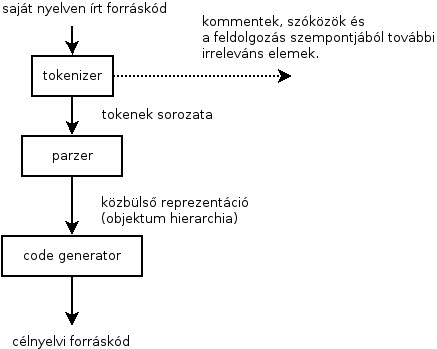
\includegraphics[scale=1]{kepek/process.png}
\caption{A keresztfordítás lépései}
\label{fig:process}
\end{figure}
A következő szakaszokban ezen lépéseknek a részletes bemutatására kerül majd sor.

\subsection{Tokenizálás}

Az tokenizálás a fordítás első fő fázisa. A felhasználó által megadott programkód beolvasását követően a nyelvi feldolgozó azt tokenek sorozatára bontja.
A token egy, a karakternél magasabb szintű logikai egységet jelöl.
A feldolgozást végző egységet ebben a fázisban angol terminológia szerint \textit{tokenizer}-nek vagy \textit{lexer}-nek (esetenként \textit{scanner}-nek) szoktak nevezni.
A tokenizer minden elemhez hozzá kell tudjon rendelni a program egy tokent, mivel a későbbi feldolgozási lépések során már csak ezek kerülnek figyelembevételre.

A tokenek sorozatában általában nem szerepelnek a különböző fehér karakterek, mint például a szóköz, újsor, tabulátor karakterek.
Ezek általában szemantikai jelentéssel nem bírnak, a kód olvashatóságát segítik.

A tokenek definiálásához a karakterek halmaza felett definiálhatunk reguláris kifejezéseket.
A leggyakrabban előforduló tokenek típusok
\begin{itemize}
\item szám literál: \texttt{[0-9\_]+}
\item szöveg literál: \texttt{[a-zA-Z0-9\_]+}
\item zárójelek: \texttt{(} és \texttt{)}
\item fehér karakterek: \verb$(\n | \r | \r | \f | \t)+$
\end{itemize}

A tokenizálás a nyelvi feldolgozás egy tipikus feladata.
Emiatt már számos olyan program elérhető, amely segíti ezen programrész elkészítését.
Ezeket lexer, tokenizer vagy scanner generátoroknak nevezzük.
A generátoroknak meg kell adni egy szintaktikai leírást, mely alapján a lexert létrehozzák, azonban figyelni kell arra, hogy az adott generátornak megfelelő módon, és az általunk megadott nyelvre illeszkedő kifejezéseket adjunk meg.

A fellelhető generátorok közül azok használata tünt szerencsésebbnek, amelyek a reguláris kifejezések segítségével adják meg a feldolgozási elemeket. Ilyenek például az \textit{AnnoFlex}, \textit{JFlex} programok, ezekről részletesebben a szintaktikai elemzéssel foglalkozó fejezetben esik szó.

\subsection{Nyelvi feldolgozás, parzolás}

A tokenek sorozata átkerül a feldolgozás következő lépéseként a parserhez.
A parzer és a tokenizer között a különbség elsősorban a feldolgozás absztrakciós szintjében van.
A parzolási folyamat szintén tipikus feladatnak tekinthető, ezért ahhoz is rendelkezésre állnak generátorok.
E mellett definiálhatunk saját rekurzív parzert is.

A lexer generátorokhoz hasonlóan a parzer generátorból is több elérhető program rendelkezésre áll.
Fontos megjegyezni, hogy olyan parzer és lexer generátort érdemes választani, melyek a lehető legjobban együtt tudnak műküdni.
Ilyen például a \textit{JFlex} és a \texttt{CUPS} generátor, mely generátort úgy terveztek, hogy egymással együttműködve tudnak működik.
A dolgozathoz elkészített program szempontjából ez a tervezettnél több problémát okozott.
Ez elsősorban a generátor programok verzióinak egyeztetéséből, és a nem túl naprakész dokumentációból adódott.

A nyelvi feldolgozás eredményeképpen egy objektum-hierarchia jön létre.

\subsection{Kód generálás}

A keresztfordítás utolsó lépése az, hogy az objektum-hierarchierarchiából ismét egy szöveges leírási mód jöjjön létre (már a cél programozási nyelven). A konvertálás tulajdonképpen abból áll, hogy a hierarchiában szereplő objektumok az adott programozási nyelvnek megfelelően tudják visszaadni magukat szöveges formában.

% ==============================
\Chapter{Célnyelvek áttekintése}
% ==============================

\section{A célnyelvek általános jellemzői}

A dolgozat szempontjából célnyelvnek azon magasszintű programozási nyelveket tekintjük, melyekre a felhasználó által, a definiált nyelven írt kód a program futtatásának végén lefordul. A program jelenleg nem minden magasszintű programozási nyelvre képes fordítani, tehát nem minden magasszintű programozási nyelv tekinthető célnyelvnek, valamint jelenleg a célnyelvként tekintett magasszintű nyelvek nem minden nyelvi elemét támogatja a program.
A további programozási nyelvek támogatása, illetve a nyelvek összes elemének a támogatására vonatkozó tervek már későbbi fejlesztési lehetőségként szerepelnek csak.
A következő szakaszokban a dolgozat szempontjából kiemelt fontosságú célnyelveket vizsgáljuk meg röviden.

\subsection{C}

A C nyelv magasszintű, általános célú programozási nyelv, mely az egyik legelterjedtebb programozási nyelv.
A ma fellelhető számítógép architektúrák szinte mindegyikére készült C fordító.
A nyelv sturkturált és szabványos programozási nyelv.
Megtalálhatóak benne azok a vezérlési szerkezetek, mint a magassabb szintű nyelvekben.
A nyelv erősen típusos, tehát változó deklarálásakor meg kell adni annak nevét és típusát.
A változó neve konvenció alapján betűvel kezdődik és utána betűket és számokat tartalmazhat.
Ezután egyenlőségjellel adhatjuk meg a változó értékét.
C nyelven az utasításokat a sor végén \texttt{;}-vel zárjuk le.
Mivel az egyes utasítások lezárását \texttt{;} jelzi, a nyelven a sortörések kihagyhatók, ezek a fehér karakterek csak az olvashatóságot növelik az esetek jelentős részében, így a fordítás során eltávolítására kerülnek.
C nyelven írt programok esetében is az utasítások szekvenciálisan futnak le.

A nyelv nem támogatja közvetlenül az objektum orientált programozás, azaz osztályok definiálására nincs lehetőség a nyelvben.
Jelen dolgozat további nyelveiben megjelenik ez a lehetőség, osztályba szervezhető a kód, mint az újonnan definiált saját programozási nyelvben is.
Emiatt komplikáltabb annak a C nyelvre történő fordítása.
C nyelvben a struktúrák találhatók meg, melyek a \texttt{struct} kulcsszóval hozhatók létre.
Ebben adhatók meg az osztályokhoz hasonló programelemek. Szintén fontos különbség, hogy a C nyelvben megjelennek a mutatók, melyek egy adott változó címét tároló változók. Ezáltal érték szerint és cím szerint is át lehet adni paramétereket.

C nyelvben emellett használható a szelekció, azaz az elágazás, mint vezérlési szerkezet.
Ezt az \texttt{if} kulcsszó vezeti be, ami után \texttt{(} és \texttt{)} között kell megadni az elágazás feltételét.
Itt a rendszer azt vizsgálja, hogy a megadott feltételek igaz vagy hamis értékűek-e, és a szerint fut le az adott ágban megírt kód. A szelekció többi ágat az \textit{else if}, illetve az \texttt{else} kulcsszó vezeti be.
A C nyelv is ismerni a \texttt{switch} szelekciót, itt is meg kell adni egy kifejezést és a \texttt{case}-en belül megadni azon kifejezéseket melyekre az illeszkedést a program vizsgálni fogja.

Emellett a programban megadható iteráció is. Ciklusból a nyelvben 3 különböző van, a \texttt{while}, \texttt{for} és \texttt{do while}. Ezek mindegyikéhez kell egy ciklusváltozó, egy feltétel, melyet minden egy ciklusban ellenőriz a rendszer. A \texttt{for} és a \texttt{while} elöl tesztelő ciklus, míg a \texttt{do while} hátul tesztelő, azaz az egyszer biztos le fog futni a cilkusmag, míg az előző kettőben nem biztos. A C nyelvben nincs külön hibakezelés, minden ilyen feladatot a programozónak kell feltételvizsgálattal megoldania, illetve klasszikus esetben nincs automatikus szemétgyűjtő algoritmus sem, vagyis a memória felszabadításáról is a programozónak kell kezeskednie.

\subsection{JavaScript}

A JavaScript egy scriptnyelv, mely leggyakrabban a böngészőkben jelenik meg, és kliens oldalon is látható a kódja. A nyelv először \textit{MochaScript} néven került definiálásra, majd később a szintaxisa a Java nyelvhez lett hasonló. Ezt követően lett a neve JavaScript.

A nyelv népszerűségét elsősorban az adja, hogy ez volt az első olyan nyelv, amelyet a legtöbb webböngésző natívan támogatott, így a \texttt{HTML} oldalakhoz alkalmazáslogikát lehetett létrehozni. Eleinte főként HTML kódba ágyazva fordult elő, majd később alakították úgy, hogy teljes értékű programozási nyelvként használható legyen.

A JavaScriptben is megtalálhatók az ismert vezérlési szerkezetek, ugyanúgy használható az értékadás, szekvencia, szelekció és iteráció is. A nyelv magasabb szintű olyan tekintetben, hogy a nyelvben már objektumok vannak. A JavaScriptben külön kifejezéssel lehet változót deklarálni, ez a \texttt{var} kulcsszó segítségével oldható meg, amelyet a változónév követ.

Külön meg kell említeni a láthatóságot a JavaScript esetében. Itt a változók alapértelmezetten csak az adott hatókörben elérhetők, ahol létre lettek hozva. Általános esetben mindenképpen egy függvény kerül megírásra, és ebben történik a változók létrehozása, a műveletek elvégzése. A változók csak az adott függvényen belül láthatók ahol létre lettek hozva. Megadhatók azonban olyan módon is a változók, hogy máshonnan is elérhető legyenek, ekkor a függvényen kívül kell deklarálni őket, így globális változókká válnak és elérhetők. Másik módszer ha olyan változóknak adunk értéket amik még nincsenek is deklarálva. A JavaScript ebben az esetben létrehozza a változót, mely azonban globális változóként kerül létrehozásra.

A nyelvben a függvények létrehozására a \texttt{function} kulcsszót használhatjuk. A nyelv megengedi a függvények értékként való átadását.

A JavaScript esetében minden utasítássort \texttt{;}-vel kell lezárni a C jellegű szintaxisa miatt, és többi formai jellegzetességében is sok hasonlóságot mutat a C nyelvvel.

\subsection{Python}

A Pyhton egy objektum orientált programozási nyelv, mely egyre nagyobb teret hódít egyszerű kezelhetősége és rugalmassága miatt. Guido van Rossum a nyelv megalkotásakor a fent emlíett egyszerűséget tartotta a legfontosabbnak.

A nyelv dinamikusan, de szigorúan típusos nyelv, tehát itt sem kell megadni típusmegjelölést.
Fontos különbség a többi nyelvhez képest, hogy nem szokás használni a \texttt{;}-t az utasítások lezárásakor, így az utasítások végét a sor vége jelenti. Azon nyelvek közé tartozik, amelynél általában nem lehet az egész programokódot egy sorban megadni, mert a formázás szemantikai jelentéssel bír.

Emellett szintén fontos különbség a blokkokat jelző \texttt{\{} és \texttt{\}} hiánya.
A nyelv az olvashatóságot is segítendő behúzásokkal jelzi az egyes blokkokat.

Általánosságban egy adott metódus, osztálydefiníció, elágazás, megírásakor a sor végére \texttt{:}-ot teszünk, ezután a következő sortól behúzással történik az adott feltétel vagy osztály magjának leírása.

A nyelv támogatja az objektum orientált programozást. A \texttt{class} kulcsszóval bevezetve osztályokat lehet megírni, melyben definiálhatunk adattagokat, metódusokat majd példányosíthatjuk azokat.

\subsection{PHP}

A PHP egy szerveroldali nyelv, tulajdonképpen scriptnyelv. Az így megírt fájlok futtatásához PHP fordítót kell telepíteni és konfigurálni.

Érdemes kiemelni a PHP hiba, illetve figyelmeztetés kijelzését is, mely szerver oldalon, az Apache konfigurációs fáljában, illetve a PHP fájlban is letiltható, illetve engedélyezhető. Érdemes ezt mindig engedélyezni a fejlesztés során, mivel egyéb esetben egyes hibák elfedésre kerülnek a PHP rugalmassága miatt, így a végső eredmény is hibás lehet. Például az alábbi kódban:
\begin{cpp}
<?php
   function multiply ($value) {
      $value = $value * 10;
      return $value;
   }
   
   $retval = multiply();
   Print "Return value is $retval\n";
?>
\end{cpp}
Látható, hogy a \texttt{multiply} függvény egy paramétert vár, és azzal számol, azonban a meghívásakor nem kerül átadásra paraméter. Ilyenkor a PHP rugalmassága miatt, egyszerűen 0 értékkel fog számolni a program, azaz a végeredmény is nulla lesz.

Azonban ez nyilvánvalóan nem a helyes működés lenne (kivéve természetesen, ha pont a 0 számmal szeretnénk meghívni egyébként is a metódust), ezért érdemes bekapcsolni a hibajelzést. Ilyenkor a program kijelzi, hogy bár a metódus deklarálásakor megadtuk, hogy paramétert várunk, meghívásakor nem adtunk neki paramétert.

Általánosságban a PHP megvalósítása miatt, ha ilyen hibákat vétünk (és ha nincs hiba kijelzés) a PHP mindig megpróbálja megoldani, kísérletet tesz a program lefuttatására.

A PHP alapvetően nem objektum orientált nyelv. Eredetileg ez szerveroldali scriptnyelv volt, csak a 2004-ben kiadott 5-ös verzióval került be az objektum orientáltság. Mivel a PHP akkoriban a legnépszerűbb szerveroldali scriptnyelv volt, nagyon sok olyan kód készült, melyben objektum orientált leírás nem volt, így ezeket először át kellene alakítani objektum orientálttá.

\subsection{Java}

A Java nyelven megírt kódok futtatásához is saját környezet kell. A java futtatókörnyezet elérhető minden elterjedt operációs rendszerre. Az egyik leginkább elterjedt programozási nyelv, amelynek egyaránt ok az, hogy szerver oldalon szivesen használják, illetve hogy a mobil alkalmazások esetében az Android platform is támogatja.

A Java nyelvben, ha bármilyen hibát vétünk akkor arról remélhetőleg már a kód fordítása során értesítést kapunk. A fordítás ekkor leáll. Tekintsük például az alábbi Java kódot.
\begin{java}
public class Test {
    private value;
    
    Test(int value) {
        this.value = value;
    }

   public void multiply() {
      value = value * 10;
      System.out.println("Return value is: " + value);
   }

   public static void main(String args[]) {
      Test test = new Test();
      test.multiply();
   }
}
\end{java}

Ez a kód már fordításkor hibát fog jelezni, hiszen a konstruktorban zárójelpárban megadtuk, hogy várunk egy integer értéket, viszont a main függvényben az osztály inicializálásakor nem adtunk azt meg. 

\section{Célnyelvek összehasonlítása}

Az alábbi részben a tervezett célnyelvek szintaxisának, elemeinek áttekintése történik meg a hangsúlyt az egyes célnyelvek különbözőségeire fektetve.

\subsection{Nyelvi típusok}

Az alábbiakban egy összefoglaló látható a különböző nyelvi típusokról (\ref{tab:lang_types}. táblázat), hogy az egyes célnyelvekben megjelenik-e az adott típus és ha igen akkor milyen formában. Ez alapján egy áttekintést kaphatunk arról, hogy a megírt kód lefordítása után az egyes nyelveket a típusok hogyan jelennek meg.
A kapott táblázat alapján meg tudjuk majd állapítani, hogy mely típusok jelennek meg a nyelvek nagy többségében, azaz a fordítás során mely típusokat kell mindenképpen figyelembe venni, megvalósítani.

Mivel a programozási nyelv megalkotása és a fordító megvalósítása során mindvégig a könnyű használhatóság és egyszerű megtanulhatóság fontos szempontként szerepelt, ezért jelen verzióban csak a fent említett közös típusok kerülnek megvalósításra. A későbbiekben ez bővíthető, úgy hogy az egyes célnyelvek minden elemét tudja a program kezelni.
\begin{table}
	\centering
	\begin{tabular}{c|c|c|c|c}
		\textbf{C} & \textbf{Python} & \textbf{Java} & \textbf{JavaScript} & \textbf{PHP}\\
		char & - & - & string & string \\
		unsigned char & - & char & - & - \\
		signed char & - & - & - & A -> - \\
		int & int & int & number & integer \\
		unsigned int & - & - & - & - \\
		short & - & short & - & - \\
		unsigned short & - & - & - & - \\
		long & - & long & - & - \\
		unsigned long & - & - & - & - \\
		float & - & float & number & float vagy double \\
		double & inf & double & number & float vagy double \\
		long double & - & - & number & - \\
		void & - & void & - & - \\
		array & array & array & array & array \\
		pointer & - & - & - & - \\
		structure & class & class & object & object/class \\
		- & str & string & string & string \\
		- & boolean & boolean & boolean & boolean \\
	\end{tabular}
	\caption{Programozási nyelvi típusok}
	\label{tab:lang_types}
\end{table}

% TODO: Általános hivatkozásokat berakni az adott programozási nyelvekhez!

A táblázatból látható, hogy a C nyelvben alapvetően sok különféle típus került definiálásra, melyek a további nyelvekben vagy nem jelennek meg, vagy ha meg is jelennek, közös típus alá vannak rendelve, azaz egy-egy típust kell csak megjeleníteni a kódban.

Külön érdemes kiemelni a PHP, JavaScript és a Python nyelveket, melyeknél az egyszerű típusokat nem is kell megjeleníteni a kódban, az adott változó típusát mindig az aktuális értéke határozza meg. Bár igaz, hogy a típus az érték alapján kerül meghatározásra, ettől függetlenül az idézett dokumentációkban megjelennek az egyes típusok, hiszen a nyelvek a típusokat felismerik, függetlenül attól, hogy egy változó deklarálásakor meg kell-e adni azt vagy sem.

A fenti táblázat alapján a fordítóprogram a szám és szöveg típusú változókat támogatja, emellett a tömb, boolean és struktúra típust is. Jelenleg a további típusokat a fordítóprogram nem fogja támogatni, ezek beépítése egy további fejlesztési lehetőség lehet.

A szám típusok közül jelenleg az integer típus támogatott, mivel ez a leggyakrabban használt az általunk vizsgált témakörben, a szöveg string típusú lesz, mivel ez a megszokott a programozási nyelvek tekintetében, csakúgy mint a boolean típus. A definiált programozási nyelv típusosság tekintetében a Python nyelvre hasonlít, így a típus megjelölése itt sem szükséges.
A tömb típust itt dictionary néven fogjuk kezelni, a struktúra pedig a modern, objektum-orientált nyelvekhez hasonlóan osztályokból fog állni, melyek a változókat illetve függvényeket foglalhatnak magukba.

\subsection{Változók deklarálása}

Az alábbi részben áttekintjük, hogy az egyes célnyelvként tekintett magas szintű programozási nyelvekben a változó deklarálásában milyen különbségeket tapasztalhatunk. Az egyes célnyelvek függően attól, hogy a típusmegjelölést ki kell-e írni, illetve, hogy milyen kulcsszóval vagy kulcsszó nélkül adjuk meg az egyes változókat nagyban különböznek. Ezt a különbséget a fordítóprogramnak kezelnie kell, és el kell fednie a felhasználó elől.

A legfontosabb különbség a C és Java nyelv illetve a Python, JavaScript és PHP hármasa között van, ahogy a különbségek nagyobb részében így lesz. A változók deklarálása során az előbbi két nyelvben minden esetben ki kell írni a változó típusát a változó neve elé, például
\begin{cpp}
	int valtozo;
\end{cpp}

Azt is megtehetjük, hogy a deklarálással együtt inicializáljuk a változót, azaz egy értéket is adunk neki. Ez minden célnyelvként vett nyelv esetében működik, azaz megtehetjük, hogy az alábbi módon adjuk meg a változót például Java nyelven:
\begin{cpp}
	int valtozo = 12;
\end{cpp}

Ezzel szemben a Python, JavaScript és PHP nyelveken a típusmegjelölést nem kell kiírni a változó elé, viszont ezen nyelvek többségében is jelezni kell, hogy egy változót adunk meg. Általánosságban ilyenkor annyit mondhatunk, hogy egy nevet rendelünk egy értékhez, hogy milyen típus lesz az, azt az érték fogja meghatározni.
\begin{cpp}
	valtozo = 12
	print(valtozo)
\end{cpp}
Ennek hátránya a nehézkes kódolvasás és javítás, főleg komplex programok esetén, mivel egy adott változó bármilyen típusú értéket felvehet, de lehetséges, hogy az adott változót használó kódrésznek egy adott típusú változóra lenne szüksége, ilyen esetben nehéz lehet megtalálni a probléma pontos forrását. Ennek kiküszöbölésére a 3.6-os Python verziótól kezdődően lehetőség van egy úgynevezett \textit{hint} megadására a változónevek után, melyben megadhatjuk, hogy terveink szerint az adott változó milyen típusú értéket fog felvenni.

\begin{cpp}
	valtozo: str = "szoveg"
	print(valtozo)
\end{cpp}

% A Pythonhoz készített ellenőrzők, például a mypy program, már képesek ezeket feldolgozni, és a Java fejlesztőkörnyezethez hasonlóan kódoláskor már jelezni az esetleges típusbeli eltéréseket. Forrás: https://medium.com/@ageitgey/learn-how-to-use-static-type-checking-in-python-3-6-in-10-minutes-12c86d72677b

A JavaSript nyelvben ismét más megoldást vezettek be a változók esetében, itt a Java nyelvhez hasonlóan deklarálni kell a változókat, azonban típust itt sem kell megadnunk. A deklarálás mikéntjének vizsgálatában ismét először nézzük meg a régebbi verziókat először. Itt még csak a \textit{var} kulcsszóval történik a deklaráció, és szokásos módon itt is azonnal értéket is tudunk adni a változónak.
\begin{cpp}
	var valtozo;
	valtozo = "szoveg";
	var valtozo2 = 12;
\end{cpp}
Az ilyen módon deklarált változók minden esetben az őket bezáró funkciókban érhetők csak el, illetve globálisan ha nincs bezáró funkció.
Az ECMAScript 2015 bevezetésekor változott ez meg, ami ECMAScript6 néven terjedt el a programozók körében. Ebben bevezettek két új váltózó típust és deklarálásukat.
\begin{cpp}
	let valtozo = "szoveg";
	const valtozo = "szoveg";
\end{cpp}
A \textit{let} esetében, nem csak a bezáró funkcióban, de azon belül is csak abban a bezáró blokkban használható, ahol deklarálva lett.
\begin{cpp}
	var valtozo = 5;
	console.log(valtozo);
	{
		let valtozo = 8;
		console.log(valtozo);
	}
	console.log(valtozo);
\end{cpp}
A fenti példában az első konzol kiíratás 5-öt fog megjeleníteni, a második 8-at, míg a harmadik szintén 5-öt. Azonban fontos megjegyezni, hogy ha így írjuk meg a kódot
\begin{cpp}
	{
		let valtozo = 8;
		console.log(valtozo);
	}
	console.log(valtozo);
\end{cpp}
akkor a második kiíratás hibára fog futni, hiszen ahogy említettük, a let kulcsszóval deklarált változó csak az adott bezáró blokkon belül érhető el.

A \texttt{const} kulcsszóval deklarált változók majdnem teljesen úgy működnek, mint a let kulcsszóval deklaráltak, azaz csak az adott blokkon belül érhetők el, azonban ezek konstansok, azaz értékük nem változik.

% TODO: Forrásokat behivatkozni!
%Forrás:
%http://es6-features.org/\#Constants,
%http://es6-features.org/\#BlockScopedVariables,
%https://www.w3schools.com/js/js\_es6.asp,
%https://www.sitepoint.com/how-to-declare-variables-javascript/

A PHP nyelv ebből a szempontban nagyon egyszerű, itt sem kell típust kiírni, és a változó deklarálásakor a név előtt egy \textdollar jelet kell megadni.
\begin{cpp}
	\$valtozo = 8;	
\end{cpp}

\subsection{Szekvenciális típusok kezelése}

A tömböket általánosságban hasonlóan kell definiálni az egyes célnyelveken, de itt is okozhatnak nehézséget a fordítóprogram megvalósítása szempontjából a kisebb különbségek is.

A C nyelvben a tömbök deklarálásához meg kell adni először a tömb típusát, majd a nevét, végül a tömb méretét \texttt{[} és \texttt{]} között. A tömböt azonnal fel is tölthetjük elemekkel, ekkor nem kell a tömb méretét külön megadni, csak az egyenlőségjel után \texttt{\{} és \texttt{\}} jel között kell felsorolni a tömb elemeit.
Ha csak az egyik elemet akarjuk módosítani akkor a név után \texttt{[} és \texttt{]} jel között meg kell adni hanyadik elemet akarjuk módosítani majd az elem értékét. A tömb mindig a 0-ás indexelésű lesz, azaz az első elem a 0. indexű.
\begin{cpp}
	int tomb[10];
	int tomb2[] = {1, 5, 10, 25};
	int tomb[2] = 4;
\end{cpp}

A Java nyelv hasonlóan működik, azzal a különbséggel, hogy a tömbök típusa után kell megadni a szögletes zárójelpárt, és a méretét csak az inicializálás során kell megadni.
\begin{cpp}
	int[] tomb;
	tomb = new int[5];
	int[] tomb2 = new int[]{3, 5, 2};
\end{cpp}
A tömbök tekintetében a JavaScript, PHP és Python elég hasonlóan működik. Mindhárom nyelv esetében meg kell adni a tömb nevét, ami egy változó lesz, majd fel kell sorolni a tömb elemeit, melyek többféle típusúak is lehetnek. Az adott tömbök futás alatt bővíthetők, tehát új elemet hozzá lehet adni a tömbökhöz. Ez utóbbival vigyázni kell, mivel egy adott változó direkt módon egy adott helyre történő beillesztése a tömbbe akár lyukakat is hagyhat a tömbben.

JavaScript alatt az alábbi módon valósítható meg a tömb kezelése:
\begin{cpp}
	var tomb = ["egy", "ketto"];
	console.log(tomb[1]);
	tomb[2] = "harom";
	tomb.push("harom");
	consloe.log(tomb.length);
\end{cpp}

% tomb[2] = "harom"; //Nem ajánlott használat
% tomb.push("harom"); //A tömb végére illeszti az elemet
% consloe.log(tomb.length); //Tömb méretének lekérdezése

Ugyanez a tömbkezelés Python alatt lista használatával:
\begin{cpp}
	tomb = ["egy", "ketto"];
	print(tomb[1]);
	tomb.append("harom");
	print(len(tomb));
\end{cpp}

% tomb.append("harom"); //A tömb végére illeszti az elemet
% print(len(tomb)); //Tömb méretének lekérdezése

Végül a kezelés PHP alatt az alábbi lesz:
\begin{cpp}
	$tomb = array("egy", "ketto");
	echo $tomb[1];
	$tomb[2] = "harom";
	array_push($tomb, "harom");
	echo count($tomb);
\end{cpp}

% $tomb[2] = "harom"; //Nem ajánlott
% array_push($tomb, "harom"); //A tömb végére illeszti az elemet
% echo count($tomb); //Tömb méretének lekérdezése

\subsection{Ciklusok}

A célnyelvként tekintett programozás nyelvekben a ciklusok megvalósítása nagyon hasonlóan működik, minden tekintett célnyelvben van elöltesztelő és hátultesztelő ciklus is. A ciklusokban minden esetben van egy feltétel, egy ciklusváltozó, melynek változása lesz a feltétellel összehasonlítva és egy ciklusmag, mely minden iterációban lefut.

A fontos különbség a tekintett célnyelvek között, hogy maga a nyelv sajátosságai megtalálhatók itt is, tehát például a Python nyelvnél nincs a ciklusmag \texttt{{} és \texttt{}} közé téve, de természetesen függetlenül ettől ez is blokkot képez. A többi nyelvnél általában a kapcsos zárójel kiírásával megjelenítik a blokkot.

A ciklusoknak a két fajtája, a while és a for minden nyelvben megtalálható.
\begin{cpp}
	for (int i = 1; i < 10; i++) {
		System.out.println(i + "\n");
	}
	int j = 1;
	while (j < 10) {
		System.out.println(j + "\n");
		j++;
	}
\end{cpp}
A fenti példa egy Java kód a ciklusokra. A C nyelvben ez a ciklusszervezés majdnem teljesen megegyezik, a fő különbség az, hogy a C nyelvben a változókat mindig előre, a program elején kell deklarálni, tehát az nem tehető meg a ciklus fejlécében.

A Python while ciklusa azonos a fenti kódban írtakkal, természetesen a nyelvi sajátosságok miatt fennálló különbségek kivételével. A for ciklus ebben az esetben kicsit megváltozik, de így is hasonlít a Java nyelvben található foreach ciklusra, mivel ilyenkor egy listán fut végig a ciklus.
\begin{cpp}
	tomb = ["egy", "ketto", "harom"];
	for i in tomb:
		print(i)
\end{cpp}

JavaScript és PHP alatt a ciklusok majdnem teljesen megegyeznek a Java kódban látható ciklusokkal, természetesen itt is meg kell említeni a nyelvi sajátosságokat (például a PHP változók előtt itt is szerepelnie kell a \textdollar szimbólum), melyek eltéréseket okoznak és melyeket figyelembe kell venni a kimeneti kód megalkotásakor.

\subsection{Függvények}

A függvények kezelése a célnyelvekben szintén hasonlóan működnek. A függvényeknek kell legyen egy fejlécük, melyben megadjuk a nevüket, visszatérési értékük típusát (statikus típusos nyelvek esetében), és a paraméter listát, illetve szükséges egy függvénytörzs is.

A fő különbség itt a C nyelvben van, ahol a függvényeket előre definiálni kell, egy prototípust kell a program elején írni belőlük, melyben fel kell tüntetni a függvény visszatérési értékének típusát, nevét és a paraméterek típusait. Ez a C nyelv esetében azért szükséges mivel a programnak tudnia kell a függvényről a meghívás helyén, és régebbi konvenció szerint a program belépési pontja azaz a \texttt{main} függvény után írjuk a többi függvényt. Azonban ha minden függvény teljesen megírásra kerül a main függvény előtt, függvényprototípusokat nem szükséges definiálni. Ezt kihasználva a C nyelvre fordítás is egyszerűsödhet a függvények kezelése szempontjából.
\begin{cpp}
	public static void main(String[] args) {
		int i = 1;
		int j = 2;
		System.out.println(addFunction(i,j));
	}
	
	public int addFunction(int a, int b) {
		return a+b;
	}
\end{cpp}
A fenti Java kódban egy függvényt és annak meghívását lehet látni. A függvények és meghívásaik a többi célnyelvként tekintett programozási nyelven is hasonlóan működnek.

A fő különbség a Python nyelvben, hogy ott a nyelvi sajátosságok miatt általában nem kell láthatósági módosítót és visszatérési érték típust megadni, ellenben a \texttt{def} kulcsszóval kell a függvény leírását bevezetni. Meghívása a Java nyelvhez hasonlóan a függvény nevével történik. Ahogy a függvény neve elé nem kell, úgy a paraméterlistában a paraméterek nevei elé sem kell a típus megjelölés, azonban az újabb Python verziókban a fentebb említett \textit{hint} itt is használható.

A PHP esetében a különbség majdnem ugyanaz, mint a Python esetében, tehát nem kell láthatósági módosító és típusmegjelölés sem, viszont a függvényt itt is kulcsszóval kell bevezetni, ez pedig a \texttt{function} lesz a PHP esetében. A paraméterek elő itt is kell a változóknál említett \textdollar szimbólum.

A JavaScript esetében szintén ez a helyzet mint az előző két esetben, és itt is a \texttt{function} kulcsszóval kell bevezetni a függvényt.

A függvények esetében visszatérési érték is lehetséges, hiszen a függvénytörzsben elvégzett adatokkal akár vissza is térhet a függvény a meghívó függvénybe. Ezt a \texttt{return} utasítással kell megadni minden nyelvben.

Szintén érdekesség, hogy a függvények paraméterének a legtöbb nyelvben lehet egy alapértelmezett értéket adni, és amennyiben nem kap értéket a meghíváskor, akkor ezt a kezdeti értéket fogja használni.
A C nyelv ebből a szempontból sajnos kivétel, nem támogatott alapértelmezetten ez a megoldás, természetesen különböző módokon lehet olyan programot írni melyben akár struktúrákkal, akár több függvénnyel a fent leírt hatás elérhető, de ez nehézkes. A legközelebbi beépített megoldás ezzel kapcsolatban a változó paraméterekkel (\textit{varargs}) megoldott függvény lenne, de ez nem a legegyszerűbb megoldás és itt az ellenőrzések sem egyszerűek.
Ugyanígy a Java nyelv sem támogatja ezt a funkciót. Természetesen itt is megoldhatók ezek, itt a függvénytúlterhelés (\textit{function overloading}) lenne a megoldás, amely esetben több függvényt írunk ugyanazon néven különböző paraméterlistával (ezt a Java támogatja), és az egyes függvények csak meghívják a további függvényeket melyek mind több és több paramétert tartalmaznak, míg végül az eredetileg megírni kívánt függvényt is. Az egyes függvények pedig a több paraméterrel rendelkező függvényeket egy alapértelmezett paraméterrel hívják meg, így a felhasználó mindig azt a függvényt tudja meghívni amennyi paraméter éppen a rendelkezésére áll a többi pedig alapértelmezett értékekkel kerül kitöltésre. Sajnos a nagyobb függvények esetében ez is eléggé bonyolulttá teszi nem csak a kódot de az ellenőrzést és javítást is.

A JavaScript a ECMAScript 2015-től kezdődően támogatja az alapértelmezett paramétert, csakúgy mint a PHP és a Python is támogatja ezt, így ez a három célnyelv az ami a kód bonyolítása nélkül képes ezeket kezelni.

Minthogy két nyelv is van a célnyelvként választott nyelvek között mely ezt nem támogatja, ezért a rugalmasságot és egyszerűséget alapul véve a definiált nyelvben sem lesz egyenlőre ez a funkció benne, így alapértelmezett paramétereket nem tudnak a felhasználók megadni. A fordítóprogram további fejlesztésekor, a felhasználói visszajelzéseket figyelembe véve lehet kibővíteni ezzel a rendszert.

\subsection{Struktúra és osztály definiálása}

Általánosságban a kódot a célnyelvek valamilyen struktúrába szervezik. A magas szintű, modern programozási nyelvek az osztályokba szervezést követik, azaz a kódot valamilyen szempont alapján különböző osztályokba szervezik és ezek együttműködnek a program futása során.

A dolgozat szempontjából célnyelvként vizsgált nyelvek szinte mindegyike támogatja az osztályokba szervezést, kivéve a C nyelvet, melyben máshogy lehet ehhez hasonló szerkezetet megoldani.
\begin{cpp}
	public class Osztaly {
		int a;
		
		public Osztaly(int a) {
			this.a = a;
		}
	
		public int getA() {
			return this.a;
		}
	}
\end{cpp}
A fenti rövid Java nyelven írt példa mutatja be az osztályokat. A vizsgált célnyelvek közül a C nyelvet kivéve az osztályok megalkotása ehhez hasonlóan működik, minden osztálynak kell egy neve legyen, adattagjai és metódusai. Java nyelven az osztálynak egy láthatósági módosítója is van. Az adott nyelveken az osztályoknak van egy kiemelt metódusuk, a konstruktor. A Java nyelven ez az osztály nevével ellátott függvény lesz, melynek nincs visszatérési értéke, ez inicializálja a változókat, melyeket osztályon belül adattagnak nevezünk. Java nyelven lehetőség van több konstruktort is írni a fentebb említett method overloading segítségével, így egy osztály többféle módon is példányosítható lesz.
A példányosítás után az egyes metódusokra (amennyiben elérhetőek) a \texttt{.} operátorral hivatkozhatunk.

JavaScript nyelven az osztály tulajdonképpen egy egyedi függvényként is tekinthető, azaz a megírt tartalom függvényként is definiálható lenne. Azonban az osztályban történő definiálás az áttekinthetőség és az egyszerűbb leírás miatt történt. JavaScriptben is a class kulcsszóval kell bevezetni az osztálydefiníciót, azonban láthatósági módosítót nem kell megadni hozzá. Itt is létezik konstruktor függvény, de itt a constructor néven kell megírni, és csak egy darab lehet belőle. A példányosítás után itt is a \texttt{.} operátorral hivatkozhatunk az osztály metódusaira, adattagjaira.

PHP nyelven szintén a class kulcsszóval kell bevezetni az osztály deklarálását, viszont itt különbség, hogy a konstruktort a \texttt{\_\_constuct} függvény néven kell megírni. Az osztály metódusaira és adattagjaira viszont itt a \texttt{->} operátorral lehet hivatkozni.

A Python nyelven az előzőekhez hasonlóan szintén class kulcsszóval kell az osztályt létrehozni, viszont itt is másik néven szerepel a konstruktor, itt az \texttt{\_\_init\_\_} függvényt kell megírni, melyet a nyelvi sajátosságok alapján a def kulcsszóval kell bevezetni. A metódusokra és adattagokra itt is a \texttt{.} operátorral lehet hivatkozni.

Ahogy fentebb említésre került, a C nyelv nem obejtum orientált nyelv, azaz osztályokat nem lehet definiálni, ezért ilyen esetben kerülő megoldás kell. A C nyelvben definiálhatunk struktúrákat, azonban itt problémát jelenthet, hogy a metódusokat nem tudjuk magában a struktúrában definiálni, azaz külön kell azokat definiálni és explicit átadni neki magát a struktúrát, hogy az adattagjait kezelni lehessen. Emiatt a program eléggé bonyolulttá válhat, könnyen összekeverhető, hogy melyik struktúrához mely függvények tartoznak. Ennek kivédésére különböző névkonvenciókat alkalmazhatunk. Viszont jelen dolgozat esetében nem kell a felhasználónak ilyennel foglalkoznia, hiszen a definiált nyelven megírt kódot a program fordítja le, így az állítja össze a célnyelvi megfelelőjét. Viszont sajnos ilyenkor ha a kimeneti programot tovább szeretné a felhasználó szerkeszteni akkor az nehézségeket okozhat, de mivel a bemeneti programot lehet a továbbiakban is szerkeszteni ezért a kimeneti fájlt nem szükséges szerkeszteni.
Az alábbiakban látható egy példa a C nyelven megírt osztályhoz hasonló program megvalósításra.
\begin{cpp}
	typedef struct osztalyDef {
		int a;
		int b;
	} osztaly;
	
	int osztaly_getA(osztaly* osztPeldany) {
		return osztPeldany->a;
	}
	
	int osztaly_getB(osztaly* osztPeldany) {
		return osztPeldany->b;
	}
	
	void osztaly_setA(osztaly* osztPeldany, int x) {
		osztPeldany->a = x;
	}
	
	void osztaly_setB(osztaly* osztPeldany, int x) {
		osztPeldany->b = x;
	}
	
	int osztaly_addNumber(osztaly* osztPeldany) {
		return osztPeldany->a + osztPeldany->b;
	}
	
	osztaly osztDef;
	
	int main()
	{
		osztaly_setA(&osztDef, 10);
		osztaly_setB(&osztDef, 5);
		
		printf("%d", osztaly_addNumber(&osztDef));
		
		return 0;
	}
\end{cpp}

% ===========================
\Chapter{A nyelv definíciója}
% ===========================

\section{Általános szempontok}

A saját nyelv kialakításánál az elsődleges szempont a könnyű kezelhetőség volt, hogy bár több nyelvre, több platformra kerülhet lefordításra a kód, a felhasználó, programozó egyszerűen, könnyen tudja megírni a kódot a definiált nyelven, így nem kell minden célnyelvi szintaktikai és szemantikai szabállyal tisztába lennie, azokat külön-külön alkalmaznia.

Ezek alapján a nyelv a Python nyelv szintaktikájához hasonló megoldásokat és jegyeket hordoz magán, a nyelvi szintaktika és szemantika megvalósításának tekintetében.

Ahhoz, hogy a nyelvet definiálni lehessen az alábbiakban áttekintjük a feladat során célnyelvként tekintett nyelveket általánosan, azok megvalósítását, tulajdonságait, fő elemeit. Majd ezután a saját definiált nyelv tervezett nyelvi elemeit vesszük sorra.

\section{Saját nyelvi elemek}

A saját nyelv definiálásakor a fentiek alapján az alábbi nyelvi szintaktika kerül kialakításra.
A definiált nyelvben is a megadott konstrukciók végrehajtási sorrendjét a vezérlési szerkezetekkel szabályozhatjuk, melyek az értékadásokon kívül a szekvencia, szelekció és iteráció.

A nyelvben az értékadás a Python nyelv egyszerűségét idézi, azaz meg kell adni egy változó nevét és az értékét. Ahogy az utasítások sorának végére, ide sem kell ;-t tenni.

Az értékadást az alábbi példa szemlélteti:
\begin{cpp}
string szoveg = "szoveg"
\end{cpp}

A változók definiálásakor meg kell adni a változó típusát, mivel a nyelv erősen típusos. A nyelv az \textit{int}, \textit{string}, \textit{double}, \textit{boolean}, \textit{void}, \textit{array} és \textit{dictionary} típusokat ismeri, melyek minden tekintett célnyelvben megtalálhatók, a C nyelvben a string karaktertömbként, illetve a dictionary struktúraként, így mindegyik nyelvre lehet fordítani.
\begin{cpp}
int valtozo1 = 5
string valtozo2 = "szoveg"
string valtozo3 = valtozo1 + valtozo2
\end{cpp}

% int valtozo1 = 5 ~ szám típusú
% string valtozo2 = "szöveg" ~ text/string tipusú
% string valtozo3 = valtozo1 + valtozo2 ~ eredmény 5szöveg, mint string típusú változó

A változók, illetve osztály adattagok esetében meg lehet adni láthatósági módosítót is, azonban ez nem kötelező. Ha nincs megadva láthatósági módosító egy adott változóhoz, akkor a nyelvi definicíó alapján alapértelmezetten private láthatóságú lesz a változó, azaz csak az adott osztály, amiben a változó létre lett hozva, az tudja majd kezelni, kívülről nem lehet.

Ha azt szeretnénk, hogy kívülről is lehessen kezelni az adott változót, akkor mindenképpen ki kell írni a láthatósági módosítót. Ilyen esetben public módosítót kell megadni, így mindenhonnan elérhető az adott változó. A metódusok belül létrehozott változók minden esetben a metódusokon belül használhatók.

Az alábbi példában az látható, hogy egy tömbben különféle típusú értékek szerepelhetnek.
\begin{cpp}
array valtozoT = {1, 2, 3, 5, "tizenketto"}
\end{cpp}
A tömb elemeire a \texttt{valtozoT(x)}-el lehet hivatkozni, amely a \texttt{valtozoT} tömb \texttt{x}-edik elemét jelöli.
Túlindexelés esetén a porogramozónak figyelnie kell, ugyanis a nyelv rugalmassága miatt nem fog hibaüzenetet kapni. Ha a tömb 10 elemű és a \texttt{tomb(12)}-t hívjuk akkor a változóba ahol az elemet letároljuk, vagy metódusba ahova átadjuk egy 0 kerül át.
\begin{cpp}
array tomb = valtozoT + "husz"
Print(tomb) ~ eredmeny: 1 2 3 5 tizenketto husz
Del(tomb)
array tomb = valtozoT
tomb(2) = 1.25
tomb(3) *= 5
Print(tomb) ~ eredmeny: 1 1.25 15 5 tizenketto
Del(tomb)
array tomb = valtozoT
Print(tomb(7)) ~ eredmeny: 0
Del(tomb)

array tomb = valtozoT + {5, "nyolc", "miskolc"}
valtozoT += {5, "nyolc", "miskolc"}
Print(tomb)
Print(valtozoT)
\end{cpp}

% array tomb = valtozoT + {5, "nyolc", "miskolc"} ~a már letárolt, névvel ellátott tömbhöz egy névtelen tömböt fűzünk hozzá, ez önmagában nem tárolódik a memóriában, csak az új változóban az eredeti tömbbel együtt, ahhoz hozzáfűzve
% valtozoT += {5, "nyolc", "miskolc"} ~ ugyanaz mint az előbb, csak itt nem jön létre új változó, a már meglévőhöz kapcsolódnak az új elemek
% Print(tomb) ~ eredmény: 1 2 3 5 tizenkettő 5 nyolc miskolc
% Print(valtozoT) ~ eredmény: 1 2 3 5 tizenkettő 5 nyolc miskolc

A második vezérlési szerkezet az elágazás. A definiált nyelvben a szelekció az \texttt{If} kulcsszóval kerül bevezetésre, melyet egy feltétel követ. A feltétel három tagból kell, hogy álljon, mely egy operátor és annak két oldalán valamilyen kifejezés kell, hogy legyen.

Az elágazás további ágait \texttt{ElIf} kulcsszóval vezetjük be, mely után szintén egy feltétel kell, hogy álljon, melynek a szerkezete az \texttt{If} feltételével megegyező kell, hogy legyen. Illetve egy utolsó ág van fenntartva arra az esetre, hogy ha a szelekció egyik korába ágának feltétele sem teljesül ezt az \texttt{Else} kulcsszóval kell bevezetni, itt nem kell feltételt megadni.

A szelekció egyes ágain több végrehajtható művelet is helyet kaphat, melyeket a program sorrendben, szekvencia alapján végez el. Az egy adott ághoz tartozó műveleti blokkot a programnyelvben nem kell külön zárójel, illetve kapcsos zárójelpárral körülzárni, a definiált nyelvben az egy adott blokk határait blokk kezdetét és végét jelentő speciális utasítások megjelenése mutatja. Az \texttt{If} esetében az \texttt{If} után az \texttt{ElIf} vagy \texttt{Else} kulcsszavak lesznek ezek, az \texttt{Else} végén pedig egy \texttt{End} utasítás kell, hogy helyet kapjon.
\begin{cpp}
If elso == 1
	masodik = elso/2
	harmadik = elso-masodik
EIf elso == 2
	masodik = elso-1
	harmadik =  elso+elso
Else
	If elso == 42
		masodik = elso/2
	Else
		masodik = elso-20
	End
End
\end{cpp}

A szelekció másik típusa a definiált nyelvben olyan elágazás, mely az elágazás elején vár egy változót vagy kifejezést és ezt utána a megadott elemekre próbálja illeszteni. Ezen szelekció a \texttt{Switch} kulcsszóval kerül bevezetésre, melyet követ a változó, illetve kifejezés.

A program futása során az a kódrész fog lefutni, amelyhez tartozó elemre a kifejezés illesztése sikeres volt. Ha nincs ilyen elem akkor egy alapértelmezett kódrészként megadott kód fog lefutni, melyet a \texttt{Def} kulcsszóval kell bevezetni. Ezen kódrész megírása mindenképpen szükséges.

Az egy adott blokkba tartozó kódot ebben a szelekcióban is a kulcsszavak megjelenése. Az alábbiakban látható erre egy példa.
\begin{cpp}
Switch vizsgalt_elem
	eredmeny1:
		blokk1_utasitas1
		blokk1_utasitas2
	eredmeny1:
		blokk2_utasitas1
		blokk2_utasitas2
	Def:
		def_utasitas
End
\end{cpp}

A harmadik vezérlési szerkezet a definiált nyelvben az iteráció. Az iteráció itt is többféle lehet, melyeket a \texttt{For}, \texttt{While} illetve a \texttt{Do} kulcsszavakkal kell bevezetni, ezután következik a ciklusfeltétel, majd az utasításblokk.
\begin{cpp}
For a=1, a<5, a++
	utasitas1
	utasitas2
End
\end{cpp}

A ciklusfeltétel lehet:
\begin{itemize}
    \item  \texttt{a < 10} (ha a nem létezik automatikusan létrehozásra kerül 0 értékkel, minden ciklusmag lefutása utána automatikusan növekszik egyel)
    \item \texttt{a = 15, a > 10, a--} (15-el jön létre, csökken egyel minden ciklusmag lefutása után és addig fut míg nagyobb mint 10)
\end{itemize}

Függvények, a \texttt{Funct} kulcsszóval kerülnek bevezetésre, amit a függvény neve követ, majd a paraméterek listája zárójelpáron belül.
\begin{cpp}
Funct kiir (a)
	utasitas
End

Funct int add (a, b)
	c = a + b
End
\end{cpp}

A függvényeket szintén \texttt{End} kulcsszóval kell lezárni, illetve fontos, hogy a függvény mindig visszatér az utolsó utasításban előállított értékkel, mely egyrészt eltárolódhat, illetve akár el is veszhet attól függően, hogy a függvény milyen módon lett meghívva.
\begin{cpp}
q = add(5, 2)
\end{cpp}

A \texttt{q}-ba a fenti add függvény \texttt{c} értéke kerül, tehát 7, viszont ha a \texttt{q} és \texttt{=} törlésre kerül a kódból, a függvény így is lefut, és vissza is tér a 7 értékkel, de az nem tárolódik le sehol, tehát el fog veszni.

Az osztályok segítségével lehet jól leképezni a valóságban lévő, vagy valósághoz közel álló elemeket is. Nem csak az egyes tulajdonságok és adott elemhez tartozó változók egy egységben történő kezelésére lennének jók, de az egyes elemek, objektumok egymáshoz való viszonyát, leszármazást is meg lehetne ezzel oldani.

Mivel általánosságban is elterjedtek az osztály alapú, objektum orientált nyelvek, ezért a definiált nyelv is ilyen, így a programozóknak, a nyelv használóinak kényelmesebb lesz, mivel olyat nyelven tudnak használni, melyhez hasonlót már használtak, vagy tanultak róla.

Az osztályok a \texttt{Create} kulcsszóval kell bevezetni, majd az osztály neve következik és a paraméterek listája. Az osztályon belül a paraméterek és metódusok definiálása történik, az osztály végét az előzőekhez hasonlóan itt is az End kulcsszó jelöli.
\begin{cpp}
Create osztalynev(parameterek)
	belso parameterek definialasa
	egyedi metodusok definialasa
End
\end{cpp}

\begin{cpp}
Create osztaly
	
	Osztaly(int param1, string param2)
		int @param1 = param1
		string @param2 = param2
	End
		
	Fuct int @decPar1()
		@param1--
	End
\end{cpp}

A fenti példában látható, hogy az osztálynak meg kell adni egy konstruktort, melyben megadhatunk paramétereket is. Azokat nem kell külön előre definiálni, az a konstruktorban történik meg és itt értéket is lehet nekik adni, ha szeretnénk. Fontos, hogy az osztály saját elemeit, adattagjait \texttt{@} jellel kell megjelölni. Az osztály adattagjainak \textit{getter} és \textit{setter} metódusa automatikusan létrejön, tehát meghívható.

Az osztály változónak módosítása a \textit{getter}, \textit{setter} metódusokon keresztül lehetséges például \texttt{osztaly.getParam1}/\texttt{osztaly.setParam1} metódus meghívásával. Ugyanígy lehet meghívni saját magunk által írt metódust is.

Egy osztály és azon elemei a memóriában addig maradnak míg arra hivatkozás van, ha az osztály objektuma nincs változóba letárolva, akkor nem marad meg. A ciklusváltozó, ha a ciklusban lett létrehozva akár automatikusan akár manuálisan akkor megszűnik a ciklus végén, a memóriából is törlődik. A programban definiált változók és tartalmuk a program futásának végéig a memóriában maradnak, azután törlődnek. Illetve manuálisan is törölhetők a \texttt{Del}(változónév) segítségével, ekkor törlésre kerül a memóriából az elem.

Ha egy elemre úgy hivatkozunk, hogy nem volt még definiálva, akkor automatikusan létrejön a változó 0 értékkel, ha előtte már volt definiálva és kitöröltük, majd úgy hivatkozunk rá, akkor is 0 értékkel jön létre, bármilyen típusú értéke is volt előzőleg, erre figyelni kell.

\section{Nyelv definiálása}

\subsection{EBNF}

Az alábbiakban a programozási nyelv nyelvtanának felírása történik meg Kibővített Backus-Naur Forma és szintaxis diagram segítségével.

\begin{verbatim}
Program  ::= Class+
Class ::= "Create" Identifier LParen Identifier+ RParen
          ("ex" Identifier)? (Assignment | Function)+ "End"
Function ::= "Funct" LParen Identifier+ RParen (Assignment |
             Instruction | Selection | (For | While))+ "End"
For ::= "For" Condition Block+ "End"
While ::= "While" Condition Block+ "End"
If ::= "If" Condition Block ("EIf" Block)* ("Else" Block)? "End"
Switch ::= "Switch" (Identifier ":" Block)+ "Def" ":" Block "End"
Block ::= Expression+
Expression ::= (Instruction | Assignment)
Condition ::= Identifier Operator
              (Identifier | Character | String | Digit)
Instruction ::= Identifier "=" BinaryOperator+
Assignment ::= Identifier "=" (Character | String | Digit)+
Identifier ::= Character (Character | Digit)+
BinaryOperator ::= Identifier Operator Identifier
String ::= '"' Character+ '"'
Character ::= [a-zA-Z]+
Digit ::= [0-9]+
Whitespace ::= " " | "\n" | "\r" | "\r\n" | "\t"
Operator ::= "+" | "-" | "*" | "/" | ">" | "<" | "<=" | ">=" | "==" |
             "&&" | "||" | "+=" | "-=" | "*=" | "/="
LParen ::= "("
RParen ::= ")"
Comment  ::= '/*' ( [^*] | '*'+ [^*/] )* '*'* '*/'
\end{verbatim}

\subsection{Szintaxis diagramok}

A következő ábrákon az egyes nyelvi elemek szintaxis diagram megfelelői láthatók. (Az operátorok nem szerepelnek benne, mivel azok egyszerű felsorolásként megadható, hasonlóképp a \texttt{Whitespace} karakterekhez.)

\begin{figure}[h!]
\centering
\includegraphics[scale=0.6]{kepek/rr_comment.png}
\caption{Comment}
\label{fig:rr_comment}
\end{figure}

\begin{figure}[h!]
\centering
\includegraphics[scale=0.6]{kepek/rr_whitespace.png}
\caption{Whitespace}
\label{fig:rr_whitespace}
\end{figure}

%\begin{figure}[h!]
%\centering
%\includegraphics[scale=1]{kepek/rr_operator.png}
%\caption{Operator}
%\label{fig:rr_operator}
%\end{figure}

\begin{figure}[h!]
\centering
\includegraphics[scale=0.6]{kepek/rr_digit.png}
\caption{Digit}
\label{fig:rr_digit}
\end{figure}

\begin{figure}[h!]
\centering
\includegraphics[scale=0.6]{kepek/rr_character.png}
\caption{Character}
\label{fig:rr_character}
\end{figure}

\begin{figure}[h!]
\centering
\includegraphics[scale=0.6]{kepek/rr_string.png}
\caption{String}
\label{fig:rr_string}
\end{figure}

\begin{figure}[h!]
\centering
\includegraphics[scale=0.6]{kepek/rr_block.png}
\caption{Block}
\label{fig:rr_block}
\end{figure}

\begin{figure}[h!]
\centering
\includegraphics[scale=0.6]{kepek/rr_binaryoperator.png}
\caption{BinaryOperator}
\label{fig:rr_binaryoperator}
\end{figure}

\begin{figure}[h!]
\centering
\includegraphics[scale=0.6]{kepek/rr_identifier.png}
\caption{Identifier}
\label{fig:rr_identifier}
\end{figure}

\begin{figure}[h!]
\centering
\includegraphics[scale=0.6]{kepek/rr_expression.png}
\caption{Expression}
\label{fig:rr_expression}
\end{figure}

\begin{figure}[h!]
\centering
\includegraphics[scale=0.6]{kepek/rr_assignment.png}
\caption{Assignment}
\label{fig:rr_assignment}
\end{figure}

\begin{figure}[h!]
\centering
\includegraphics[scale=0.6]{kepek/rr_instruction.png}
\caption{Instruction}
\label{fig:rr_instruction}
\end{figure}

\begin{figure}[h!]
\centering
\includegraphics[scale=0.6]{kepek/rr_condition.png}
\caption{Condition}
\label{fig:rr_condition}
\end{figure}

\begin{figure}[h!]
\centering
\includegraphics[scale=0.6]{kepek/rr_if.png}
\caption{If}
\label{fig:rr_if}
\end{figure}

\begin{figure}[h!]
\centering
\includegraphics[scale=0.6]{kepek/rr_switch.png}
\caption{Switch}
\label{fig:rr_switch}
\end{figure}

\begin{figure}[h!]
\centering
\includegraphics[scale=0.6]{kepek/rr_for.png}
\caption{For}
\label{fig:rr_for}
\end{figure}

\begin{figure}[h!]
\centering
\includegraphics[scale=0.6]{kepek/rr_while.png}
\caption{While}
\label{fig:rr_while}
\end{figure}

\begin{figure}[h!]
\centering
\includegraphics[scale=0.6]{kepek/rr_function.png}
\caption{Function}
\label{fig:rr_function}
\end{figure}

\begin{figure}[h!]
\centering
\includegraphics[scale=0.4]{kepek/rr_class.png}
\caption{Class}
\label{fig:rr_class}
\end{figure}

\begin{figure}[h!]
\centering
\includegraphics[scale=0.6]{kepek/rr_program.png}
\caption{Program}
\label{fig:rr_program}
\end{figure}

\section{Példák}

Az alábbiakban egy egyszerűbb példa forráskód részletet, melyben egy osztály és a benne lévő elemek láthatók.

\begin{verbatim}
Create Ember
	
	Ember(string nev, int kor, int irSzam, string utca, int hSz)
		string @nev = nev
		int @kor = kor
		Cim @cim = Cim(irSzam, utca, hSz)
	End
		
	Funct void @decrKor(int szam)
		While szam>0
			@kor = @kor - 1
			@szam = @szam --
		End
	End
	
	Funct string @createString()
		@nev + @kor + @cim.createString
	End
End
\end{verbatim}
		
Az alábbiakban a fenti osztály példányosítása és használatának példája látható

\begin{verbatim}
Ember pelda = Ember("teszt", 20, 1542, "Teszteles", 50)
pelda.setParam1("TesztKetto")
string ember = pelda.createString()
\end{verbatim}


\Chapter{Szintaktikai elemzés}

% TODO: Formális nyelvekkel, fordítóprogramokkal kapcsolatos könyvek hivatkozásai.

% http://www.informatik.uni-bremen.de/agbkb/lehre/ccfl/Material/ALSUdragonbook.pdf

\section{Java parser generátorok}

Az Interneten különféle parser generátorokat találhatunk, amelyek segítségével könnyebben megoldható a szintaktikai elemzés.
A feladat megoldásához olyan parser generátorra van szükség, mely Java nyelvű, mivel a fordítóprogram ezen a nyelven kerül megírása.
Továbbá, a parser generátorok feldolgozás szempontjából is különböznek, és jelen feladathoz olyan generátort kellett keresni, mely reguláris nyelvvel képes működni.
Az alábbiakban néhány, elterjedt generátort vizsgálunk meg.

\subsection{AnnoFlex}

Az \textit{Annoflex} egy Java alapú generátor, mely szabadon letölthető és használható, sőt módosítható is.
Az AnnoFlex tervezésekor törekedtek az egyszerűségre. A következő kódrészletben láthatunk egy példát a használati módjára.
\begin{java}
/**
* @option methodName = getNextToken
* @option statistics = enabled
*/
public class Example_Annoflex {
/** @expr [0-9]+       */ String createNumber()     { return "number"; }
/** @expr [a-zA-Z]+    */ String createIdentifier() { return "identifier"; }
/** @expr [ \n\r\t\f]+ */ String createWhitespace() { return "whitespace"; }
//%%LEX-MAIN-START%%
//%%LEX-MAIN-END%%
}
\end{java}

A generátornak Java kommentekben adhatjuk meg a nyelv elemeire vonatkozó beállításokat az osztály és a metódus definíciók előtt. Az osztályra vonatkozó beállításokat \texttt{@option} formában használhatjuk. Az előző kódpéldában egyrészt a következő token beolvasásához szükséges metódus nevét adtuk meg, illetve, hogy a nyelvi feldolgozó generálása közben készítsen-e majd statisztikát a program.

Ezt követően az osztályon belül meg kell adni a kifejezéseket és a metódusokat. Itt találkozhatunk több megkötéssel is az AnnoFlex tekintetében. A megadáskor mindenképpen \texttt{@expr} kifejezéssel kell kezdeni, melyet szintén kommentben kell elhelyezni.

A kifejezés után csak és kizárólag reguláris kifejezés állhat. A komment után magát a metódust kell megírni, melynél szintén van megkötés. A metódusok nem lehetnek \texttt{static} módosítóval ellátva, visszatérési értékük nem lehet csak primitív típus vagy \texttt{String}, de mindenképpen az összes így megadott metódusnak ugyanolyan visszatérési értékkel kell bírnia, egyetlen kivétellel, ami a \texttt{void}. \texttt{void} visszatérési érték állhat más visszetérési érték mellett. További megkötés, hogy a metódusoknak nem lehet paraméterük, csak visszatérési értékük.

Minden egyes metódust csak egy darab reguláris kifejezés előzhet meg, ha több reguláris kifejezés is kellene, hogy ott álljon, akkor a reguláris kifejezések uniójával oldható ez meg, melyhez a \texttt{|} operátor használható.

Ez után következik egy tagek által határolt üres rész, ezt mindig a
\begin{java}
//%%LEX-MAIN-START%%
//%%LEX-MAIN-END%%
\end{java}
sorok határolják, és ide kerül legenerálásra magának a nyelvi feldolgozónak a kódja.

Amennyiben elkészültünk a kifejezések megírásával, akkor a fejlesztőkörnyezetben lefuttathatjuk a AnnoFlex programot.

% TODO: Itt csak behivatkozni majd valahogy a generált kódot, és csak néhány érdekesebb kódrészt mutatni belőle!

% TODO: Fel lehet sorolni a generált adattagokat és metódusokat!

% A fenti kódban látható, hogy a program legenerálta a szükséges metódusokat és funkciókat.
Ezután már nem kell mást tenni, mint egy futtatható osztályt készíteni a példához:

\begin{java}
public class Example_AnnoRun {

	public static void main(String[] args) {
		Example_Annoflex anno = new Example_Annoflex();
		anno.setString("Ez 1 teszt string");
		System.out.println("Scan:" + anno.getString());
		String token = anno.getNextToken();
		while (token != null) {
			System.out.println(token + ":" + anno.getMatchText());
			token = anno.getNextToken();
		}
	}

}
\end{java}

Ebben csak létrehozunk egy példányt az osztályból, hozzáadunk egy szöveget és lefuttatjuk a programot. A képernyőre a következő eredményt fogja a program kiírni:

\begin{verbatim}
Scan:Ez 1 teszt string
identifier:Ez
whitespace: 
number:1
whitespace: 
identifier:teszt
whitespace: 
identifier:string
\end{verbatim}

Látható, hogy \texttt{identifier}-nek jelezte a szövegeket, a számot numberként jelenítette meg és megtalálta a fehér karaktereket is, azaz a szóközöket.

\subsection{JFlex}

A \textit{JFlex} szigorú értelembe véve egy lexikai elemző, azaz lexer generátor, mely Java nyelvhez Java nyelven írt generátor. Itt is a megadott inputot próbálja meg illeszteni a különféle előre definiált nyelvtani elemekre és az annak megfelelő utasításokat hajtja végre.

A JFlex a \textit{JLex} átírt változata, melynek átírásakor a cél a teljes unicode támogatás és platformfüggetlenség volt, illetve a gyors szkenner generálás, kényelmes szintaktika és az is, hogy kompatibilis legyen a JLex-el. Önállóan is használható, de mivel főképp lexer generátor, így más parser generátorokkal történő együttműködésre tervezték, leginkább a CUP parserrel kompatibilis.

Felépítése alapján a nyelvtani specifikáció három részre osztható, melyeket a \texttt{\%\%} jel választ el. Az első a felhasználói kód, a második a beállítások és makrók része, míg a harmadik fogja tartalmazni a lexer szabályokat.

% TODO: Itt is csak említeni kellene a példával kapcsolatban néhány észrevételt!

\subsection{AustenX}

Az \textit{AustenX} (vagy röviden csak \textit{Austen}) szinten egy parser generátor. Az Austen jelenleg csak Java nyelvet támogatja, és az előzőekhez hasonlóan ez is reguláris nyelv alapján dolgozza fel a kódot.

Az Austin egy \texttt{jar} fájlként tölthető le és futtatható, aminek futtatásakor paraméterként kell megadni a célfájlt. Az Austen futtatható a jar fájlra kattintva duplán, ilyenkor egy egyszerű felhasználói kezelőfelület nyílik meg. Itt meg kell adni a forrásfájlok helyét, amiben a feldolgozáshoz szükséges adatok vannak, illetve a célfájl helyét, ahova a feldolgozott fájlok kerülnek. A forrásfájlok .austen vagy .austenx kiterjesztéssel kell, hogy rendelkezzenek. Az alábbiakban egy egyszerűbb példa látható a forrásfájlokra.

% TODO: Tömören össze kellene foglalni a generált kódot.

A generált kód egy általános leírást tartalmaz, library-k szerint szervezve melyet felhasznál az alábbi kód, ami a parser generator pontos leírását tartalmazza.

\Chapter{Közbülső reprezentáció}

A keresztfordító működése szerint beolvassa a nyelvi fájlt, melyet a programozó a definiált nyelven megírt, majd szekvenciálisan feldolgozza azt. A szinkatkikai elemzés után egy belső szerkezet jön létre, mely leírja a beolvasott programkódot.

\section{Nyelvi elemeket reprezentáló osztályok}

A kód a belső szerkezetben osztályokba lesz szervezve, ezekről az alábbiakban kerül említésre néhány információ.

\begin{figure}
\centering
\includegraphics[scale=0.2]{kepek/rr_uml.png}
\caption{Osztálydiagram}
\label{fig:process}
\end{figure}

\subsection{Függvény}

\begin{figure}
\centering
\includegraphics[scale=0.2]{kepek/rr_funccallexpr_dia.png}
\caption{Függvényhívás}
\label{fig:process}
\end{figure}

\subsection{Változó}

\begin{figure}
\centering
\includegraphics[scale=0.2]{kepek/rr_var_dia.png}
\caption{Változó osztály}
\label{fig:process}
\end{figure}

\subsection{For ciklus}

\begin{figure}
\centering
\includegraphics[scale=0.2]{kepek/rr_for_dia.png}
\caption{For ciklus osztálya}
\label{fig:process}
\end{figure}

\subsection{Elágazás}

\begin{figure}
\centering
\includegraphics[scale=0.2]{kepek/rr_if_dia.png}
\caption{Feltételes elágazás, If osztálya}
\label{fig:process}
\end{figure}

\subsection{Osztály}

\begin{figure}
\centering
\includegraphics[scale=0.2]{kepek/rr_class_dia.png}
\caption{Osztály leírása osztályban}
\label{fig:process}
\end{figure}

\subsection{Program, modul, csomag}

\begin{figure}
\centering
\includegraphics[scale=0.2]{kepek/rr_prog_dia.png}
\caption{Program osztály}
\label{fig:process}
\end{figure}

\subsection{Kód blokk}

\begin{figure}
\centering
\includegraphics[scale=0.2]{kepek/rr_block_dia.png}
\caption{A keresztfordítás lépései}
\label{fig:process}
\end{figure}

\subsection{Kifejezés}

% TODO: Jó sok UML diagram

% TODO: Absztrakt gyár mintát érdemes lesz majd bemutatni a kimeneti programnyelvek implementációjánál.

\Chapter{Célnyelvre fordítás}


\chapter*{Összefoglaló}

% Ki kellene választani majd 5-10 algoritmust, amelyikhez egy-egy szakaszban szerepelnek az implementációk, utána pedig az egyes nyelvekre való fordítással kapcsolatos észrevételek, futási idők.

A dolgozatban egy új programozási nyelv definiálására került sor. Ehhez a kiinduló pontot azok a már elterjedt, általános programozási nyelvek adták, melyek a keresztfordító szempontjából célnyelvnek tekinthetők. A nyelv definiálása során a dolgozat bemutatta, hogy milyen formában lehet leírni egy programozási nyelvet. A grafikus leírás esetében ez a szintaxis diagramokat jelentette, míg a szöveges leíráshoz a Backus-Naur Forma egy konkrét szintaxisa került felhasználásra.

Egy teljesen általánosan használható keresztfordító létrehozására vonatkozóan a fontos ismérvek részletezésre kerültek a dolgozatban. A keresztfordítás nagyobb fázisait, mint a lexikális elemzést, a közbülső reprezentáció létrehozását, illetve az ebből való célnyelvi visszaírást egy nagy feldolgozási folyamat részének tekintettem. Ezek külön fejezetekben kaptak helyet. Azt igyekeztem hangsúlyozni, hogy minden ilyen feldolgozási lépés függetlennek tekinthető olyan értelemben, hogy a jól definiált be- és kimeneteinek köszönhetően réteges szerkezetű keresztfordítót kapunk, melyek rétegei így külön fejleszthetők, tesztelhetők.

Ahhoz, hogy a létrehozott programozási nyelv népszerű lehessen még rengeteg további munkára van szükség. A dolgozat ennek mindössze az első nagy lépését mutatja be, vagyis felveti a nyelv szükségességét, majd bemutatja a keresztfordítók témakörét, egy új keresztfordító létrehozásának a folyamatát. Mivel a célnyelvek száma nagy (amire a feladat célkitűzését tekintve szükség is volt), az egyes célnyelvek sajátosságainak kezelése további fejlesztéseket igényel. A jövőbeli tervek között szerepel, hogy egy teljesen általánosan használható, széles körben elterjedt nyelv váljon a bemutatott, sajátos programozási nyelvemből.

\chapter*{Summary}

In this work, I have defined a new programming language. It is based on the analysis of the programming languages which were selected as target languages from the aspect of the cross compiler. The methods and tools of the definition of a programming language also has presented. In the case of graphical representation the grammar has described by syntax diagrams, while the textual representation has solved by the Extended Backus-Naur Form.

I have described all of the main aspects of crosscompiler design and implementation. The three important phases of the cross compilation process (namely the lexical analysis, the intermediate representation and the serialization of the target language) has considered from the viewpoint of the overall cross compilation process. These are described in separate chapters. I have tried to emphasize that these steps can be separated and results a layered architecture. It assumes well-defined input and output formats, and makes possible the development and testing of the layers independently.

For making the programming language proper for daily use for the wider audience, a large amount of further development is required. This work only present its first significant step. It reveals the requirement of this language, introduces the topic of cross compilers and the process of cross compiler design and implementation. The number of target languages are large (by the original goal of this work), the handling of language specialities requires more consideration in the future. The long term plan is to form the introduced language to a general purpose, widely used programming language.


\Chapter{CD-melléklet tartalma}

A szakdolgozatom mellé egy darab CD tartozik, amelyen a következő fájlok és jegyzékek találhatók.

\begin{itemize}
\item \texttt{szakdolgozat.pdf}: A szakdolgozat PDF formátumban.
\item \texttt{forras/}: A szakdolgozat \LaTeX\ forráskódját tartalmazó jegyzék. 
\item \texttt{crosstranslator/}: Az elkészített programok forráskódjait tartalmazó jegyzék, benne a szükséges \texttt{jar} fájlokkal, és kapcsolódó nyelvi leírásokkal.
\item \texttt{osszefoglalo.pdf}, \texttt{osszefoglalo.tex}: A dolgozat magyar nyelvű összefoglalása PDF és szerkeszthető \LaTeX\ formában.
\item \texttt{summary.pdf}, \texttt{summary.tex}: Angol nyelvű összefoglaló
\end{itemize}


\begin{thebibliography}{x}
\addcontentsline{toc}{chapter}{\bibname}

\bibitem{compilers}
Principles of Compiler Design

\bibitem{formalis}
Formális nyelvek és automaták

\bibitem{annoflex}
Stefan Czaska: \emph{AnnoFlex}, Annotation-based code generator,
\url{https://annoflex.github.io/}, 2018.

\bibitem{jflex}
\emph{JFlex The Fast Scanner Generator for Java},
\url{http://www.jflex.de/}, 2018.

\bibitem{austen}
\emph{Austen, parser generator},
\url{https://scratchy.org.nz/austen.php}, 2018.

\end{thebibliography}


\end{document}
